\section{Simulation Results}
\label{sec:simresults}

This section presents a simulation example showing how the optimization algorithm of Section \ref{sec:optimization} was used to produce a multi-domain walking gait for the planar biped AMBER 2, a planar robot that was designed and partially machined within AMBER lab at Texas A\&M University. AMBER 2 is a seven link robot supported by a light weight, carbon fiber boom that restricts motion to the saggital plane. The boom is counter weighted so as to not introduce mass to the robot; however, there is an inertial load introduced to the torso link that is negligable due to the low friction bearings used in the construction of the boom as well as a long moment arm ($\sim$ 8ft) separating the robot from the center of rotation of the boom.
\begin{figure}
\centering
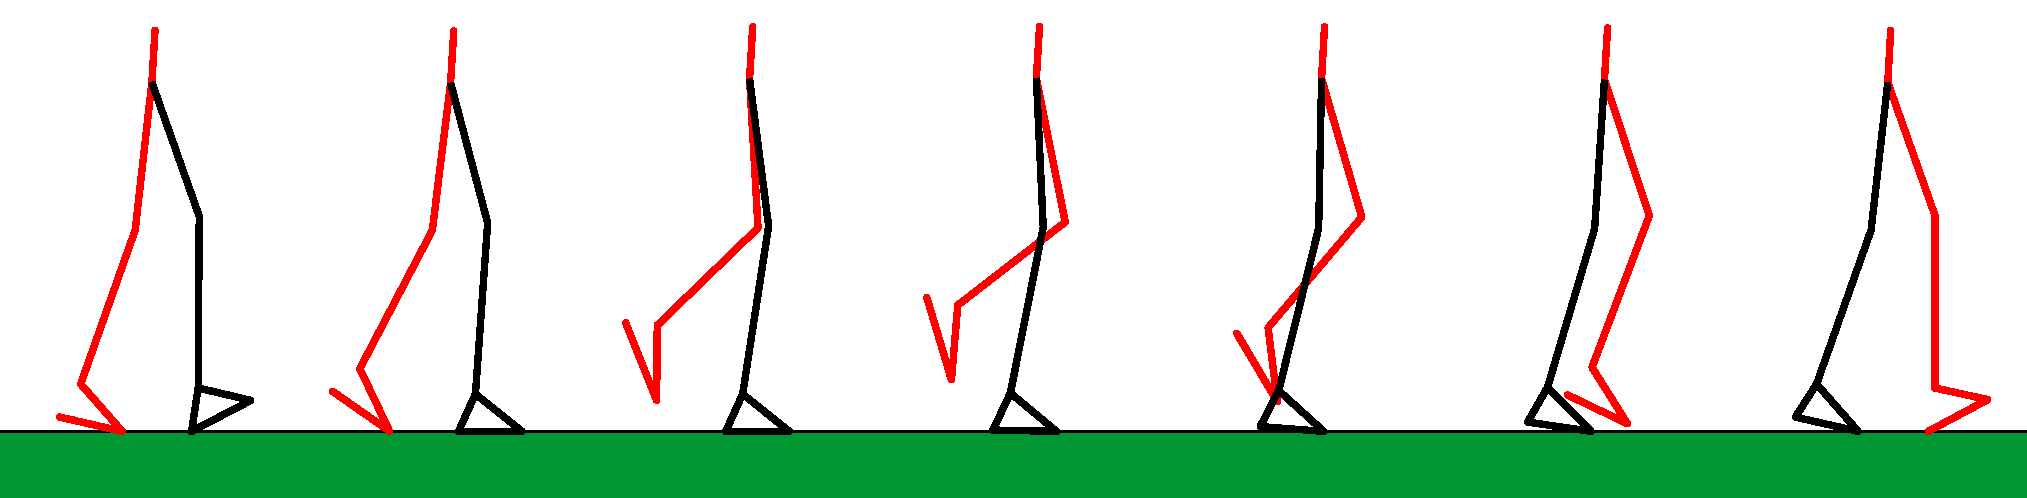
\includegraphics[scale=0.26]{figures/Tiles.pdf}
\caption{Gait tiles for a 3 domain walking gait.}
\label{fig:Tiles}
\end{figure} 
%The mass and length parameters of AMBER 2 are shown in Table \ref{table:params} with variable conventions as defined in Fig. \ref{fig:robotCoords}.
The optimization of Section \ref{sec:optimization} was implemented using MATLAB'S FMINCON function and the interior-point algorithm.
% \begin{table}[H]
% \caption{AMBER 2.0 Mass \& Length Parameters}
% \centering
% \begin{tabular}{c c c c}
% \hline\hline
% Link & Mass(g) & Length(mm) & Width(mm) \\ [0.5ex]
% \hline
% Foot & 204.42 & 177.8 & 47.63 \\
% Calf & 1119.43 & 343.13 & 50.8 \\
% Thigh & 1172.57 & 298.45 & 50.8 \\
% Torso & 2154.79 & 104.01 & 285.75 \\ [1ex]
% \hline	
% \end{tabular}
% \label{table:params}
% \end{table}
For the underactuated phase, the integration algorithm ODE45
was used to integrate the dynamics forward in time.  In both the double support and fully actuated phases, the solution at each timestep was found in closed-form using the reconstruction algorithm discussed in Section \ref{sec:reconstruction}.
\begin{figure}[t!]
\centering
\begin{subfigure}{0.001\textwidth}
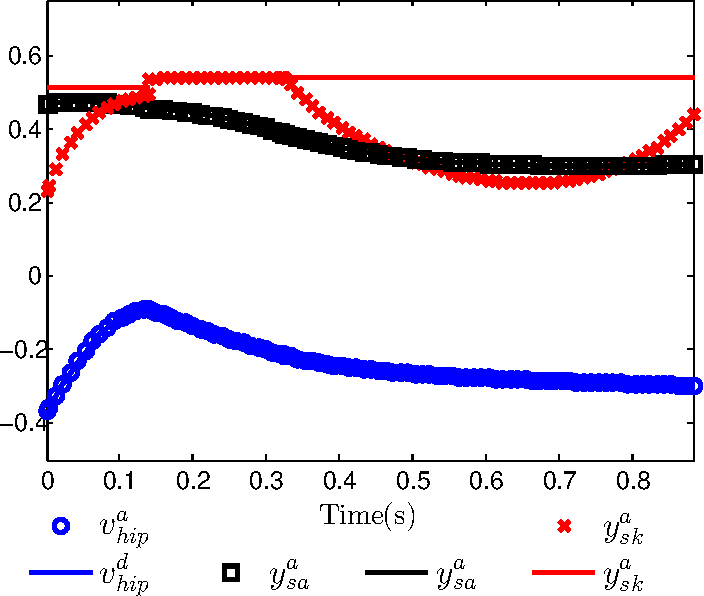
\includegraphics[width=42mm]{figures/YaVsYd1-crop.pdf}
\vspace{-42mm}
\end{subfigure}
\begin{subfigure}{0.75\textwidth}
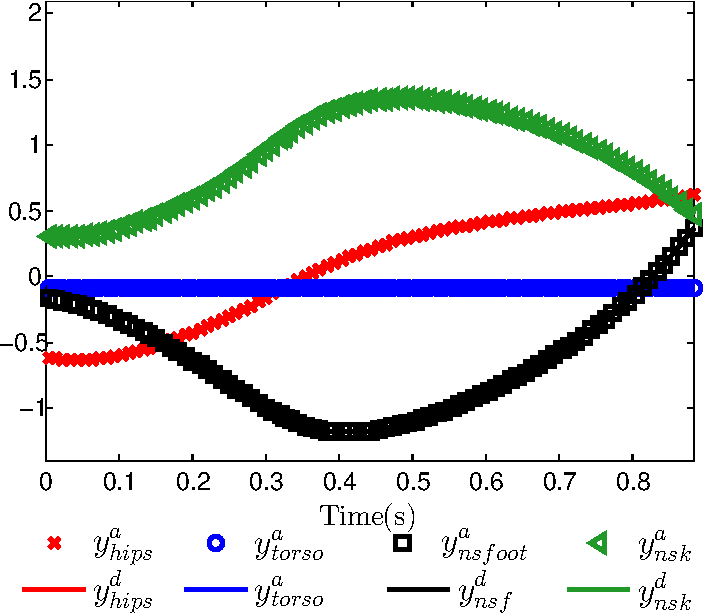
\includegraphics[width=42mm]{figures/YaVsYd2-crop.pdf}

\end{subfigure}
\caption{Actual and desired outputs over one step for a 3 domain walking gait.}
\label{fig:Outputs}
\end{figure}
The results of the optimization are shown in Fig. \ref{fig:Tiles}, where the 3-domain walking gait is plotted as a series of tiles. 
An animation is available at [\url{http://www.youtube.com/watch?v=OY-QsaIglQY}].  The gait shown here has an average velocity of 0.42 m/s, with a step length
of 0.373 m (58\% of leg length) and a period of $T = 0.88$ sec. The step time can be further broken down, with 0.139 s (16\%) in double 
support / overactuation, 0.19 s (21\%) in full actuation, and 0.56 s (63\%) in underaction. The actual and desired outputs for the gait are shown in Fig. \ref{fig:Outputs}.

The joint torques over one step with I/O Linearization and the QP are compared in Fig. \ref{fig:Torques}. Notice that for simple I/O Linearization, the torque at the nonstance ankle is identically zero for 
the domain of over actuation. This is due to the configuration of the robot only containing 5 independent degrees of freedom. With the QP, however, torques for all six actuators can be specified and, additionally, there is a decrease in the maximum required torque($\sim$33 Nm for I/O Linearization and 24 Nm for QP).
%
\begin{figure}[t!]
\centering
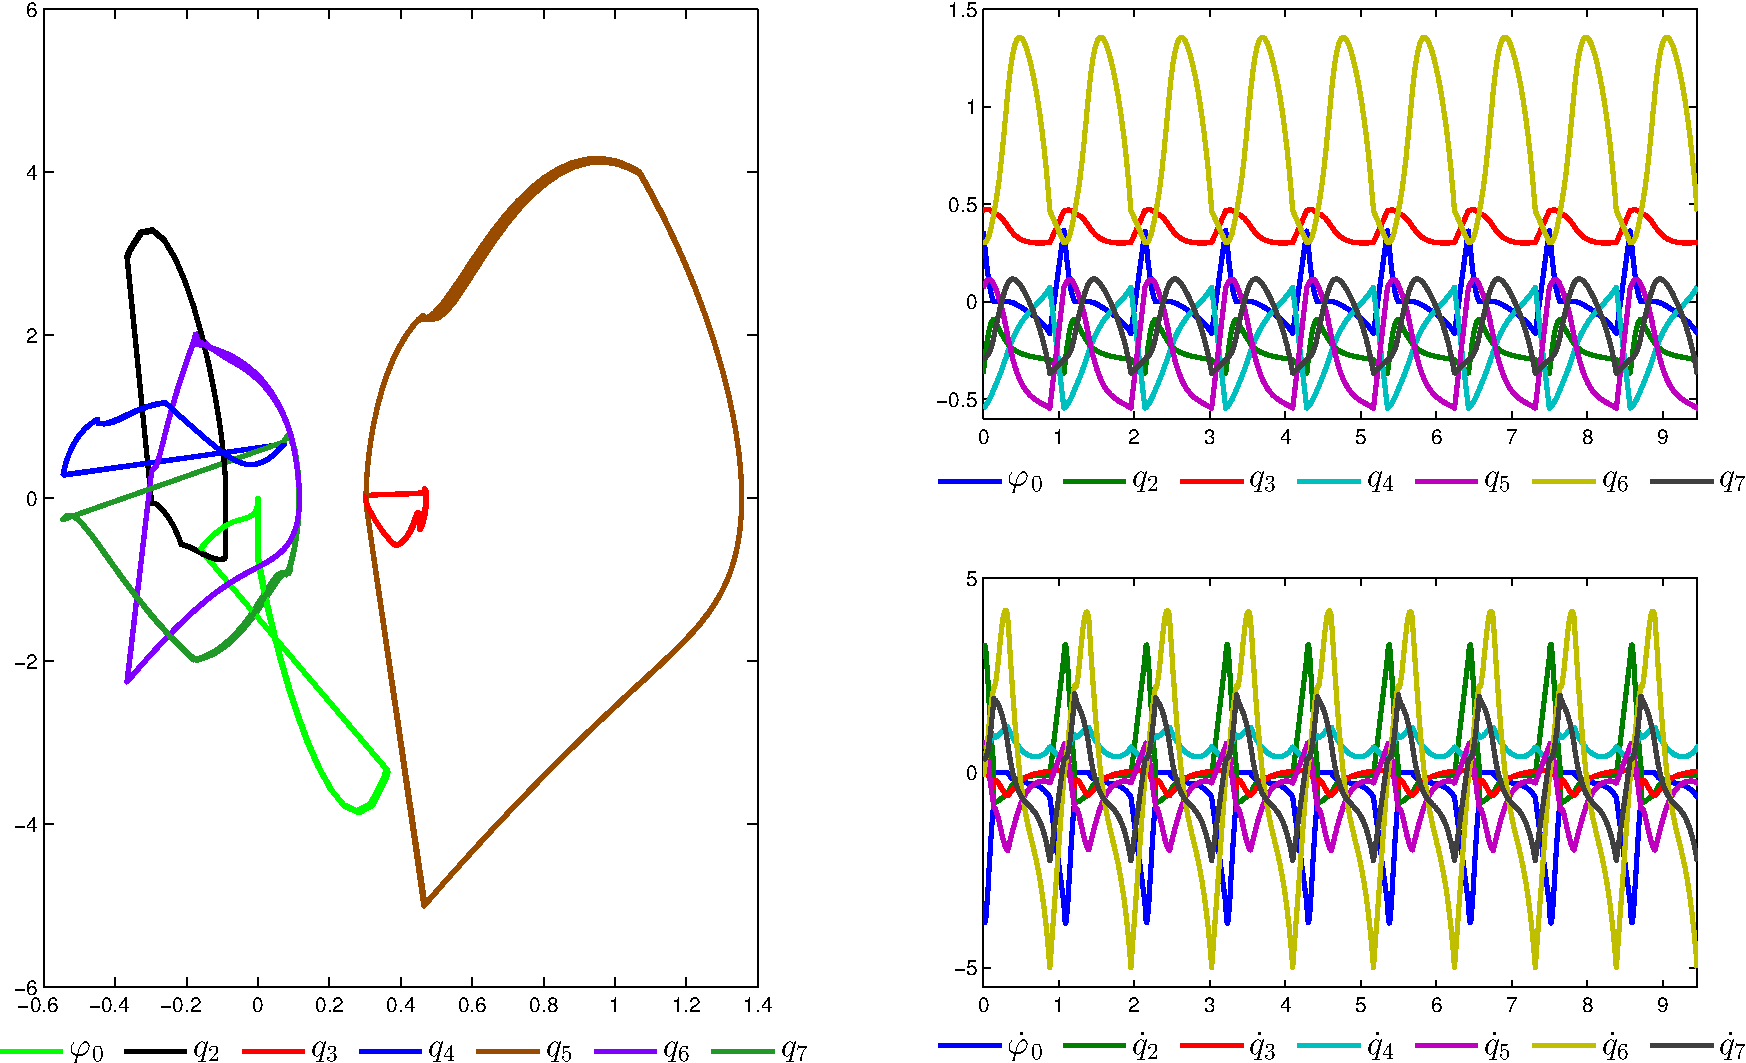
\includegraphics[scale=0.3]{figures/subplot_orbit-crop.pdf}
% \hspace{-10mm}
\caption{Phase plot (left) for 9 steps of a 3 domain walking gait showing the periodicity of the gait and joint angles (top right) and velocities (bottom right).}
\label{fig:subplot_orbit}
% \vspace{50mm}
\end{figure}
% 
\begin{figure}[t!]
\centering
\begin{subfigure}{0.75\textwidth}
\hspace{-5mm}
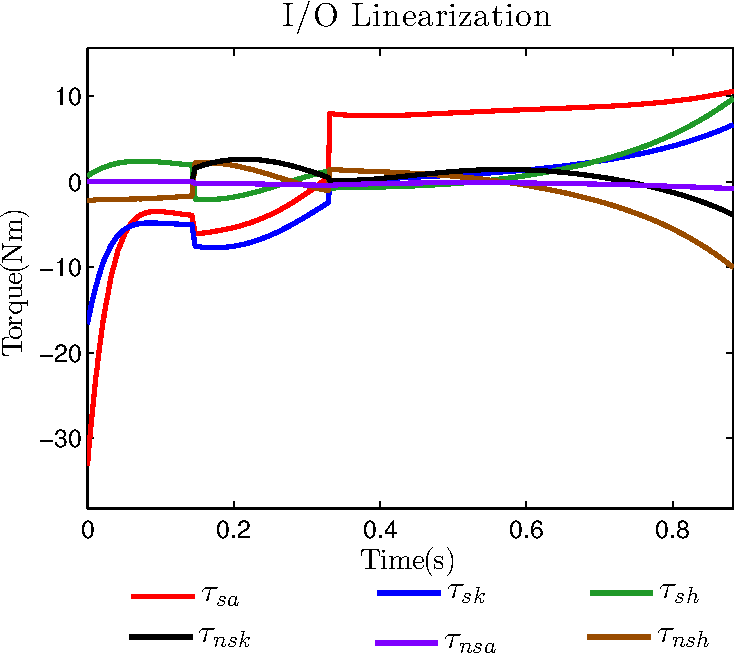
\includegraphics[width=44mm]{figures/TORK_IO-crop.pdf}
\end{subfigure}
\begin{subfigure}{0.001\textwidth}
\vspace{-39mm}
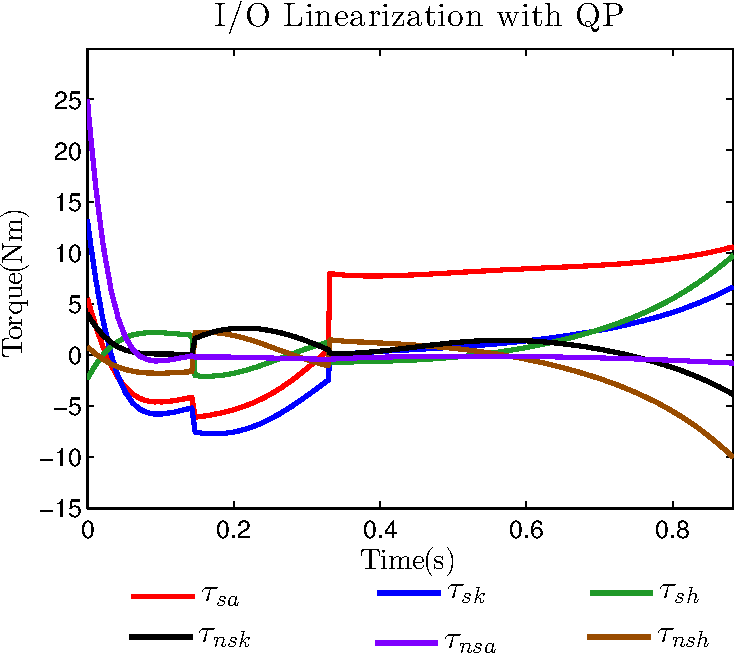
\includegraphics[width=44mm]{figures/TORK_QP-crop.pdf}
\end{subfigure}
\caption[Plots comparing joint torques from I/O Linearization and the QP.]{Joint torques over one step using I/O Linearization(left) and the quadratic program(right).}
\label{fig:Torques}
%\vspace{15cm}
\end{figure}

